%!TEX root = ../../../../exa-ma-d7.1.tex

\section{Compute distance to a range of entities}


\Cref{tab:app-feelpp-io} describes the specifications of the application.

\begin{table}[ht]
    \centering
    \begin{tblr}{
        colspec = {l X[10cm]},
        row{odd} = {numpexlightergray},
        hlines = {0.1pt, numpexgray},
        vlines = {numpexgray},
        row{1} = {numpexgray, fg=white, font=\bfseries},
    }
        Field & Details \\
        id & \texttt{app-feelpp-distance} \\
        name & Distance \\
        Partners & Unistra \\
        PC & PC1 - ExaMA, PC2 - ExaSoft \\
        Responsible (Permanent) & V. Chabannes; C. Prud'homme \\
        WP7 Engineer & Thomas Saigre (UNISTRA) \\
        work\_package & WP1 \\
        application\_type & mini-app \\
        purpose & Compute distance to a range of entities using FMM or BVH \\
        Method-Algorithm WP1 &  unstructured mesh, finite element, FMM, ray-tracing-BVH \\
        Method-Algorithm WP2 & \\
        Method-Algorithm WP3 & \\
        Method-Algorithm WP4 & \\
        Method-Algorithm WP5 & \\
        Method-Algorithm WP6 & \\
        WP7 & \\
        % inputs &  \\
        % outputs & \\
        % metrics & \\
        % status & \\
        % Benchmark scope & \\
        % Framework & \\
        % parallel\_framework & \\
        % spec\_due & \\
        % proto\_due & \\
        repo\_url & \url{https://github.com/numpex/apps-feelpp}\\
    \end{tblr}
    \caption{Description of the mini-app \texttt{app-feelpp-distance}.}
    \label{tab:app-feelpp-distance}
\end{table}


%%%%%%%%%%%%%%%%%%%%%%%%%%%%%%%%%%%%%%%%%%%%%%%%%%%%%%%%%%%%%%%%%%%%%%%%%%%%%%%%%%%%%%%%%%%%%%%%%%%%%%%%%%%%%%%%%%%%%%%%


\subsection{Description of the benchmark}

We consider the unit cube $[0,1]^3$ discretized by an unstructured tetrahedral mesh.
Let $h$ denote the mesh size, controlling the total number of vertices $N$.
For each mesh vertex $\mathbf{x}_i$, our goal is to compute the Euclidean distance
\begin{equation}\label{eq:distance-definition}
  d(\mathbf{x}_i) = \min_{\mathbf{y}\in\partial([0,1]^3)} \Vert\mathbf{x}_i - \mathbf{y}\Vert_2.
\end{equation}
The exact analytical distance on the unit cube is
\begin{equation}\label{eq:distance-exact}
  d_{\mathrm{exact}}(x,y,z) = \min\{x,\,1-x,\,y,\,1-y,\,z,\,1-z\}.
\end{equation}
We compare two numerical strategies to build a continuous piecewise-linear (P1) distance field over the mesh.

More details can be found in \cite{van_landeghem_micro-swimming_2025}.


\subsubsection{Fast--Marching Method (FMM)}
\begin{enumerate}
  \item \textbf{Initialization:} Tag all boundary vertices of the mesh as known with $d=0$.
  \item \textbf{Propagation:} Maintain a narrowband of trial vertices adjacent to known ones. Repeatedly extract the trial vertex with the minimal tentative distance, mark it known, and update neighboring trial vertices by solving local upwind discretization of the eikonal equation $\Vert\nabla d\Vert = 1$.
  \item \textbf{Output:} A P1 scalar field $d_h(\mathbf{x})$ approximating the true distance.
\end{enumerate}

\subsubsection{Ray-Tracing with BVH}
\begin{enumerate}
  \item \textbf{Preprocessing:} Build a Bounding Volume Hierarchy (BVH) over the mesh boundary faces or directly on the analytic cube faces.
  \item \textbf{Directional Sampling:} Since the cube geometry is known, but the nearest boundary direction is unknown, for each vertex $\mathbf{x}_i$ we uniformly sample directions on the unit sphere. Let $M$ be the number of rays per point, which becomes a key parameter for accuracy and cost.
  \item \textbf{Ray Casting:} For each sampled direction, cast a ray from $\mathbf{x}_i$ into the BVH and record the intersection distance. The estimated distance is the minimum over all sampled rays:
  \[ d_h(\mathbf{x}_i) = \min_{1\le j\le M} t_j, \]
  where $t_j$ is the distance along ray $j$ to the boundary.
  \item \textbf{Output:} A P1 field $d_h(\mathbf{x})$ by assigning the computed distance at each vertex.
\end{enumerate}



%%%%%%%%%%%%%%%%%%%%%%%%%%%%%%%%%%%%%%%%%%%%%%%%%%%%%%%%%%%%%%%%%%%%%%%%%%%%%%%%%%%%%%%%%%%%%%%%%%%%%%%%%%%%%%%%%%%%%%%%


\subsection{Benchmarking tools used}

Let $d_h$ be the discrete distance field computed by either method. We compute the error norms
\begin{align}
  \Vert d_h - d_{\mathrm{exact}}\Vert_{L^2} &= \left( \sum_{i=1}^N (d_h(\mathbf{x}_i) - d_{\mathrm{exact}}(\mathbf{x}_i))^2
    \right)^{1/2},\\
  \Vert d_h - d_{\mathrm{exact}}\Vert_{L^\infty} &= \max_{i=1,\dots,N} |d_h(\mathbf{x}_i) - d_{\mathrm{exact}}(\mathbf{x}_i)|.
\end{align}
We perform a convergence study over meshes with $h = h_0, h_0/2, h_0/4, \dots$, verifying that FMM yields $O(h)$ convergence, while ray-tracing achieves machine-precision at vertices.




%%%%%%%%%%%%%%%%%%%%%%%%%%%%%%%%%%%%%%%%%%%%%%%%%%%%%%%%%%%%%%%%%%%%%%%%%%%%%%%%%%%%%%%%%%%%%%%%%%%%%%%%%%%%%%%%%%%%%%%%


\subsection{Input/Output Dataset Description}


\subsubsection{Input Data:}
  \begin{itemize}
  \item Meshes: ...
  \item Setup: ...
  \item Sif image: ...
  \item ...
  \end{itemize}

Include table of figure that are relevant (size of the meshes, etc...)

\subsubsection{Output Data:}

The output includes the computed values of validation measure in CSV files format, export visualization files (mesh, partitioning, temperature), and the time taken to perform each simulation step.
Metric:
\begin{itemize}
    \item \texttt{benchmark-verification},
    \item \texttt{strong-scalability},
    \item \texttt{weak-scalability},
    \item \texttt{io-scaling}: time taken by the application to read meshes, and to write the solution on disk (especially reading).
\end{itemize}




%%%%%%%%%%%%%%%%%%%%%%%%%%%%%%%%%%%%%%%%%%%%%%%%%%%%%%%%%%%%%%%%%%%%%%%%%%%%%%%%%%%%%%%%%%%%%%%%%%%%%%%%%%%%%%%%%%%%%%%%

\subsection{Results summary}

We present in this section the results of the benchmark described above.
In \Cref{fig:specs:app-feelpp-distance:results:distance}, we show the exact distance between each point of the cube to the border.
The cube is vertically half sliced.

We also present in \Cref{fig:specs:app-feelpp-distance:results:error-bvh} and \Cref{fig:specs:app-feelpp-distance:results:error-bvh} respectively the distribution of the point wise error for the methods FMM and BVH respectively.

\begin{figure}
    \begin{subfigure}{0.33\textwidth}
        \centering
        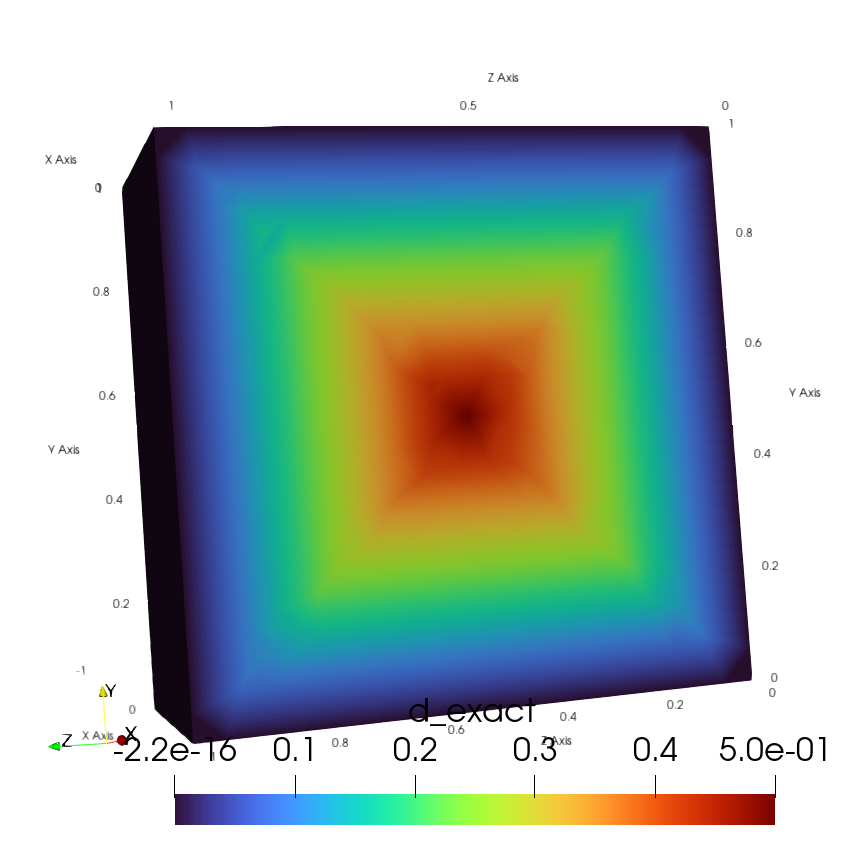
\includegraphics[width=\columnwidth]{graphics/feelpp/feelpp-benchmark-distance-exact}
        \caption{Exact distance $d_\mathrm{exact}$.}
        \label{fig:specs:app-feelpp-distance:results:distance}
    \end{subfigure}
    \begin{subfigure}{0.33\textwidth}
        \centering
        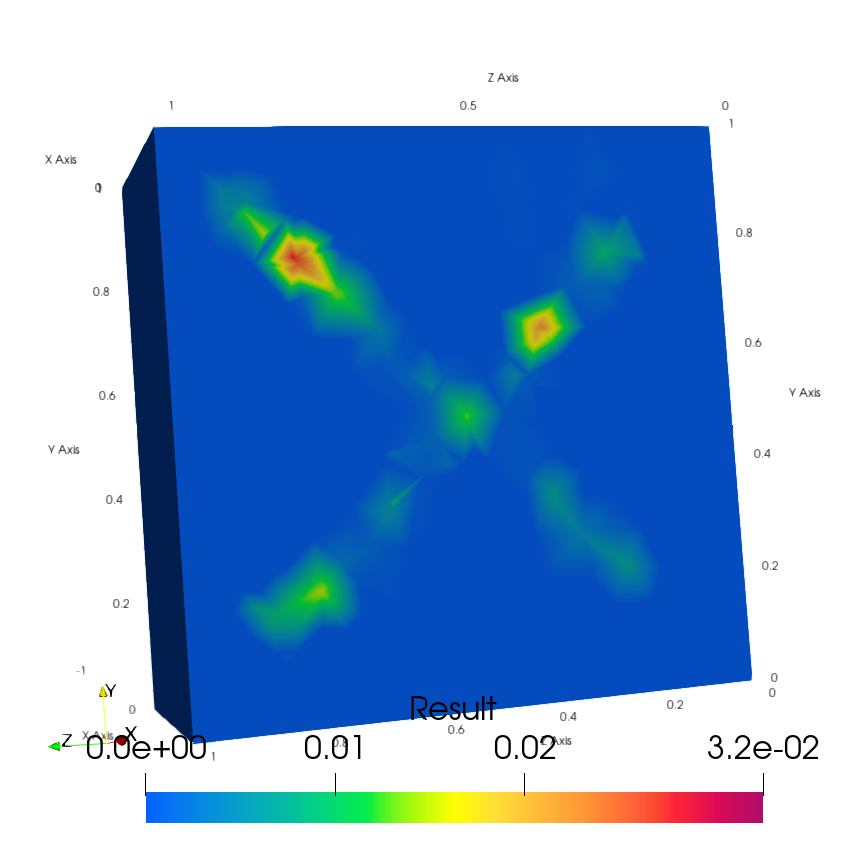
\includegraphics[width=\columnwidth]{graphics/feelpp/feelpp-benchmark-distance-errorFMM}
        \caption{Error by the method FMM: $|d_\mathrm{FMM}-d_\mathrm{exact}|$.}
        \label{fig:specs:app-feelpp-distance:results:error-fmm}
    \end{subfigure}
    \begin{subfigure}{0.33\textwidth}
        \centering
        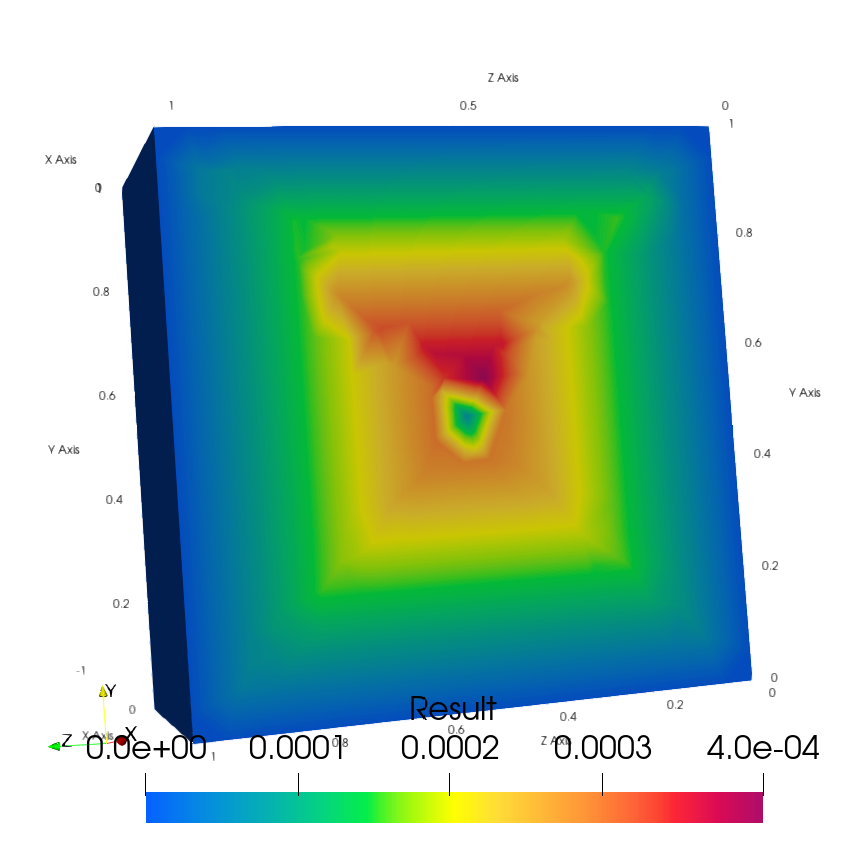
\includegraphics[width=\columnwidth]{graphics/feelpp/feelpp-benchmark-distance-errorBVH}
        \caption{Error by the method BVH: $|d_\mathrm{BVH}-d_\mathrm{exact}|$.}
        \label{fig:specs:app-feelpp-distance:results:error-bvh}
    \end{subfigure}
    \caption{Numerical results of distance computing.}
    \label{fig:specs:app-feelpp-distance:results}
\end{figure}
